\section{Einzelne Komponenten vernetzen}

Das Backendsystem von Elastifeed besteht aus mehreren einzelnen Komponenten, die erst im Zusammenschluss die gewünschte Funktionalität bereitstellen.
Zentral findet sich Elasticsearch, eine auf Lucene basierte NoSQL Datenbank die über eine REST-Schnittstelle Funktionalität zum Einfügen und Suchen von Dokumenten bereitstellt.\cite{es}

\begin{figure}[t]
        \centering
        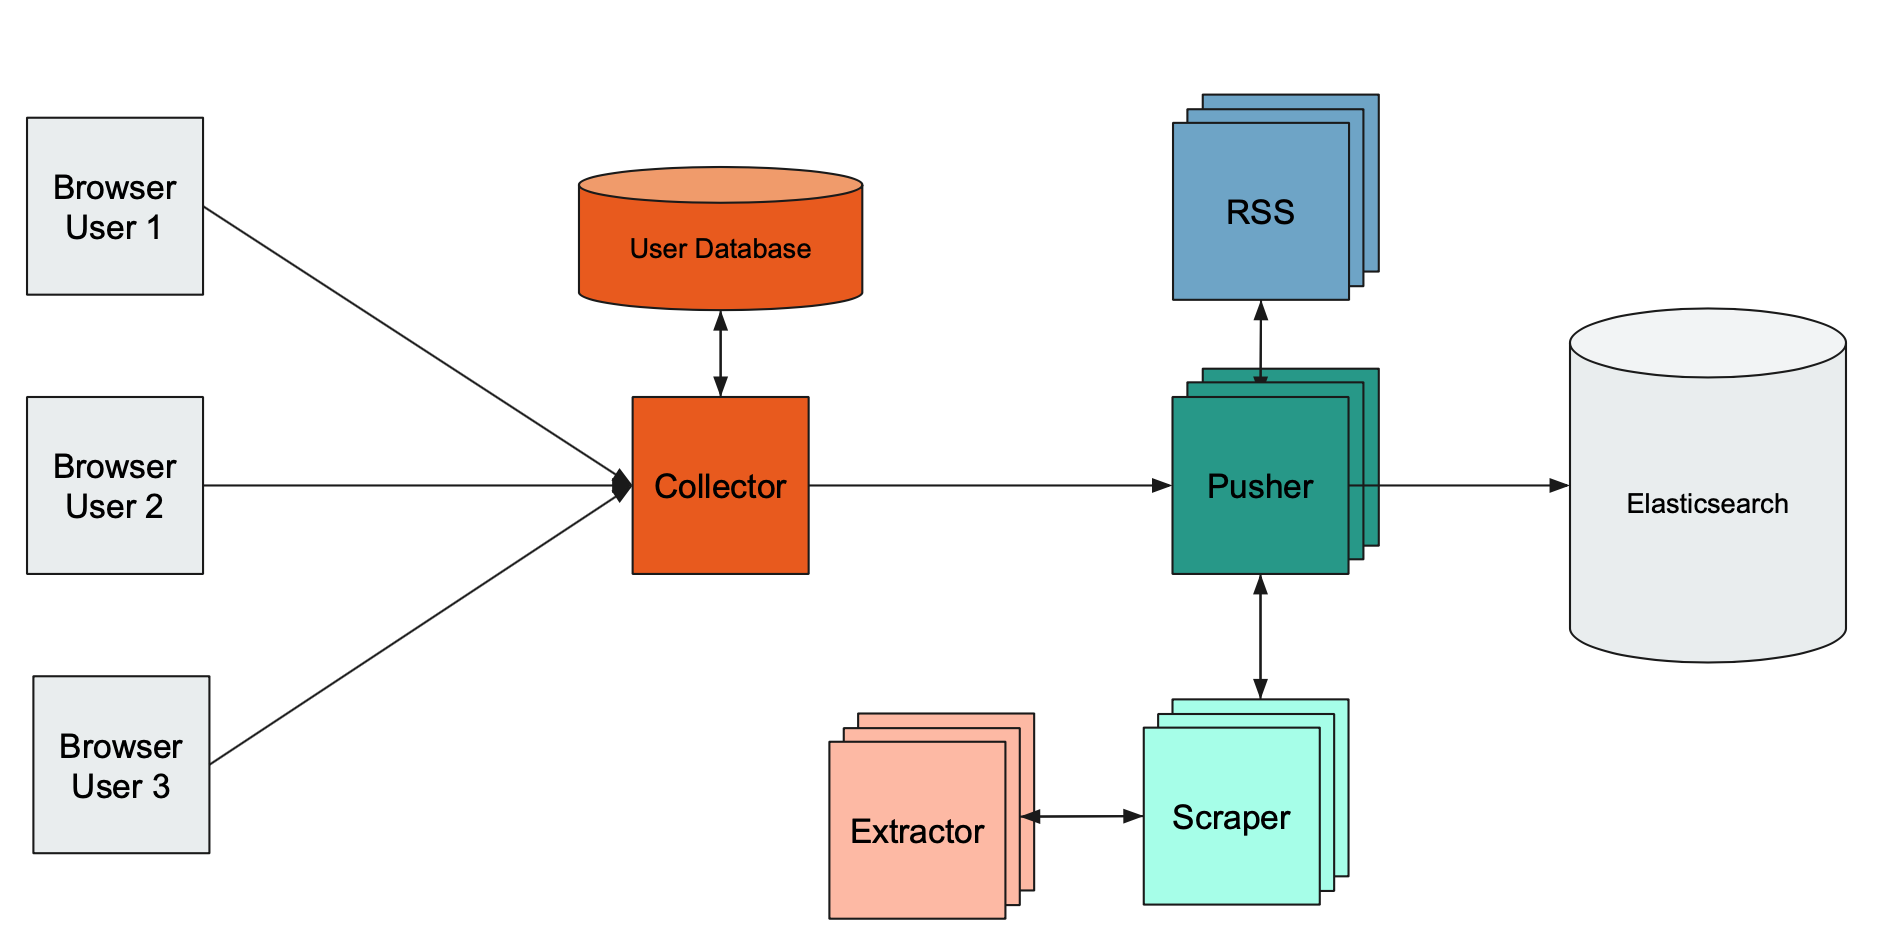
\includegraphics[width=\linewidth]{images/architecture.png}
        \caption{Zusammenhang der einzelnen Komponenten}
        \label{deploy:image:architecture}
 \end{figure}
